\documentclass[manuscript,screen,review]{acmart}
\acmJournal{TECS}
\setcopyright{none}
\settopmatter{printacmref=false}
\usepackage{tikz}
\usetikzlibrary{arrows.meta,positioning,calc,fit,backgrounds}
\usepackage{pgfplots}
\pgfplotsset{compat=1.18}
\usepackage{tabularx}
\graphicspath{{figures/}{../figures/}}
\newcommand{\protset}{\mathcal{P}}
\newcommand{\risk}{\mathcal{R}}
\newcommand{\E}{\mathbb{E}}
\newcommand{\Prob}{\mathbb{P}}
\newcommand{\bits}{\mathcal{B}}
\newcommand{\code}[1]{\texttt{#1}}
\newcommand{\clip}{\operatorname{clip}}
\definecolor{nsnavy}{HTML}{18354A}
\definecolor{nsteal}{HTML}{087E8B}
\definecolor{nsgold}{HTML}{BC771B}
\definecolor{nspale}{HTML}{EFF4F6}
% Draft markers (15 November 2026): red text is provisional evidence or a result still being computed.
\newcommand{\pending}[1]{{\color{red}#1}}
\newcommand{\waiting}[1]{{\color{red}\textbf{[Pending:} #1\textbf{]}}}
% Cross-references: the whole "Figure 3" / "Section 5" / "Eq. (4)" is the link, and links are boxed (hyperref's default
% look: red for internal links, green for citations, cyan for URLs) instead of coloured.
\newcommand{\wref}[2]{\hyperref[#2]{#1~\ref*{#2}}}
\newcommand{\weqref}[2]{\hyperref[#2]{#1~\textup{(\ref*{#2})}}}
\AtBeginDocument{\hypersetup{colorlinks=false,pdfborder={0 0 0.8},linkbordercolor={1 0 0},citebordercolor={0 0.6 0},urlbordercolor={0 0.6 0.9}}}

\title[Between Single Bits and Every Combination]{Between Single Bits and Every Combination: How Stored-Bit Faults Add Up in Quantized Neural Networks, and Which Bits to Protect\\ {\normalsize\color{red}[working title, to be decided]}}
\author{Manuel Blanco Valent\'in}
\affiliation{\department{Electrical and Computer Engineering}\institution{Northwestern University}\city{Evanston}\state{Illinois}\country{USA}}
\author{Houxuan Guo}
\affiliation{\department{Electrical and Computer Engineering}\institution{Northwestern University}\city{Evanston}\state{Illinois}\country{USA}}
\author{Xiuyuan He}
\affiliation{\department{Electrical and Computer Engineering}\institution{Northwestern University}\city{Evanston}\state{Illinois}\country{USA}}
\author{Seda Ogrenci}
\affiliation{\department{Electrical and Computer Engineering}\institution{Northwestern University}\city{Evanston}\state{Illinois}\country{USA}}
\renewcommand{\shortauthors}{Blanco Valent\'in et al.}
\ccsdesc[500]{Computer systems organization~Reliability}
\ccsdesc[300]{Computer systems organization~Embedded systems}
\ccsdesc[300]{Computing methodologies~Neural networks}
\keywords{quantized neural networks, fault injection, selective protection, embedded machine learning, stored-bit faults, reliability evaluation}

\begin{document}
\begin{abstract}
Selective protection of neural-network weights must decide which stored bits to protect. Existing rankings treat this as a single-bit problem: they order bits by significance or by the isolated effect of one flip, and so assume that the effects of simultaneous faults add up. Simulating every combination of faults is out of reach. We show that the problem lies in between. Under a protection mask, the stored-bit faults of an INT8 network behave like Gaussian noise on every weight, with the exact mean and variance of its unprotected bits, plus a few discrete events in the two most significant bits. Passed through the network, this model reproduced measured accuracy within about half a point on average on two models \pending{(exploratory; a confirmation on 18 further checkpoints is running)}. It explains what we measure on 24 checkpoints of nine architectures, from 4,000-weight MLPs to a 0.6-billion-parameter language model, with masks compared on common fault fields in the task metric. Protecting by bit significance, as FORTUNE does and as FKeras does within each significance tier, wastes the budget once faults are dense: at 12.5\% protection it loses 9 to 34 accuracy points across nine ResNet-8 checkpoints, and 24 on Visual Wake Words, where the absolute-gradient ranking loses at most 5.3. Ranking bits by the per-example magnitude of their gradient effect is a strong default. No static ranking is guaranteed. Rankings that also use the sign of a flip win at sparse faults on ResNet-8, lose up to 57 points at dense faults, and on language models can do worse than no protection; the fault rate at which the preference switches is predicted from calibration data on ResNet-8 but not on DS-CNN. The protection mechanism matters as much as the ranking. When every stored bit, including redundant copies and check bits, can fail, triplicating ranked bits beats SEC-DED codes and ABFT checksums at dense fault rates and loses to them at sparse ones \pending{(ResNet-8 and DistilBERT measured; all other models running)}.
\end{abstract}
\maketitle
\section{Introduction}\label{sec:introduction}
Which parameter bits should be protected when a neural network cannot be protected in full? Bit significance offers an inexpensive answer: suppress faults in the most significant positions first. Other methods use numerical perturbations, gradients, curvature, or measured fault effects to identify important locations. The engineering question is whether the extra information yields a better allocation under the fault probability and protection budget of interest.

The effect of a stored-bit fault depends on its encoding, location, input, and the other faults present. Consequently, a ranking that predicts isolated damage need not minimize loss when many bits can fail simultaneously. This observation does not make static protection obsolete. A fixed mask can be appropriate for a fixed operating condition, and a ranking can itself incorporate multi-fault information. What requires measurement is whether a particular allocation transfers across conditions.

We investigate this question with six frozen INT8 networks spanning vision, speech, anomaly detection, sentiment classification, and language modeling. We compare structural and gradient rankings throughout, and a published Hessian-based method where its computation has been validated. Each comparison uses the same proposed random fault fields, input cohort, eligible-bit population, and protection budget. Reliability is measured against logical bit-error probability (BER) and protected-bit fraction, not inferred from score correlations alone.

Three questions organize the evaluation: does a score predict isolated damage; does its resulting mask preserve task quality under simultaneous faults; and does the preferred allocation remain preferable when the budget or fault probability changes? These are different tests. A good answer to the first does not establish the second, and success at one operating point does not establish the third.

The contribution is a controlled comparison and its decision-level findings. Paired results reveal changes in relative method quality with model, BER, and budget. We also test whether conditioning on faulty backgrounds improves a local allocation beyond exact isolated-bit measurements. It often changes the mask, but a 32-pool KWS study does not establish a held-out improvement over that stronger comparator. This negative result limits the practical conclusion just as much as the observed ranking reversals.

Our earlier design flow included hardware synthesis and selective redundancy~\cite{guo2025inpixel}. The present study is software-only: it evaluates exact stored-code XOR faults and ideal suppression on protected coordinates. It neither measures physical mitigation overhead nor converts logical BER into a radiation rate. The intended outcome is an evidence-based choice of allocation for a declared operating condition, not another universally preferred score.

\section{Related Work and Scope}\label{sec:related}
\subsection{Sensitivity analysis and fault-injection prioritization}
FKeras analyzes the sensitivity of heavily quantized edge networks using gradients and leading weight-loss Hessian eigenpairs~\cite{weng2024fkeras}. It evaluates single- and multi-bit faults and refines parameter ordering within significance tiers. The present comparison preserves the published projection and tier ordering while adapting the continuous model and numerical solver to the frozen INT8 benchmarks. We do not equate FKeras with a diagonal-Hessian approximation or claim that it ignores cross-parameter curvature.

PrioriFI extends this line of work by using observed damage to guide subsequent fault injections~\cite{weng2026priorifi}. Hessian information initializes significance queues, and feedback determines which queue to probe next. Its endpoint is efficient discovery of sensitive fault locations. Converting that procedure into a mask of exactly $B$ protected bits introduces a further decision: how to combine observed and unobserved coordinates, how much probing to spend, and how to freeze the result before independent evaluation. NetSuRF has engineering support for studying such a conversion, but the present manuscript contains no completed PrioriFI-derived effectiveness comparison.

EISFINN uses importance sampling guided by neuron- and bit-level attribution to improve the efficiency of fault-injection campaigns~\cite{colucci2024eisfinn}. This is relevant precedent for directed exploration of faults, including an activation-level fault domain. Finding harmful events efficiently and estimating risk under a prescribed random law are nevertheless different statistical objectives. An importance-biased sample requires the corresponding probability correction before it estimates the latter. Our final evaluations retain the declared independent Bernoulli target and paired field identities.

These studies already establish that bit significance alone is an incomplete sensitivity description and that adaptive injection can be useful. Our empirical question is more specific: for frozen equal-budget masks, how does measured task risk vary with BER and coverage, and does exact conditioning improve a local protection decision beyond exact isolated measurements? The new measurements and numerical contracts, rather than the existence of nonlinearity or adaptive exploration, form the basis of the comparison.

\subsection{Selective hardening and physical mitigation}
Selective hardening has been investigated for FPGA neural networks~\cite{libano2019selective}; selective TMR can triplicate sensitive channels to meet a minimum-accuracy requirement under single channel-stuck faults~\cite{garciabertoa2023selective}. Other techniques exploit bit-level redundancy for recovery~\cite{catalan2025redundancy}. FORTUNE combines post-training affine quantization with two additional copies of each weight's MSB and majority voting during inference~\cite{nazari2024fortune}. Its precision search trades clean accuracy against reliability and resource requirements. This shares a significance preference with MSB-first allocation, but changes the representation and includes redundant storage and voting. Our fixed-checkpoint masks do not reproduce those correction mechanisms or their costs.

In particular, ideally protecting all INT8 sign bits covers 12.5\% of our eligible population, but implements neither ECC nor TMR. Ranger restricts intermediate value ranges to dampen transient datapath corruption, with protected memory assumed in its main fault model~\cite{chen2021ranger}. FT-CNN uses convolution checksums with distinct detection and correction capabilities; it also considers memory corruption and recovery through weight reloading or recomputation~\cite{zhao2021ftcnn}. These are complementary interventions, not interchangeable ranking methods. Their quantitative comparison would require matched fault domains, executable recovery behavior and verified resource costs. We therefore discuss them as related protection mechanisms without assigning their names to ideal-suppression curves.

The public \emph{Learned or Ranked?} companion release is another close precedent~\cite{alobaidi2026selectiveecc}. Its archived implementation includes matched-cost protection methods, held-out evaluation, paired layer interaction diagnostics and context-dependent layer marginal rankings. The release is cited as a dataset and source archive; peer-reviewed publication of its accompanying manuscript has not been established here. Its layer/bit-plane decisions and ideal or word-level ECC models differ from our individual-bit, fixed-cardinality interventions and reference integer execution. We do not claim the first observation of context-dependent protection, nor superiority to its allocation algorithms.

\subsection{Relationship to the earlier NetSuRF design flow}
Our FCCM work already connected susceptibility analysis, user budgets, selective TMR and an HLS-to-hardware implementation flow~\cite{guo2025inpixel}. The overall engineering motivation and the idea of using bit priorities to allocate resources are therefore inherited. This paper contributes a separate software methodology with exact encoded-state injection, explicit score-to-mask contracts, paired uncertainty, independent task-specific benchmarks, and a controlled test of isolated versus conditional decisions. Its resource axis is protected-bit count, and its measured results come from new frozen executable studies. It neither reuses the earlier hardware performance claims nor presents the general design-flow concept as new.

\section{Evaluation Workflow and Fault Model}\label{sec:fault}
The evaluation has three stages (Fig.~\ref{fig:workflow}). It freezes a trained model, its numerical execution and its task data. It builds protection masks from calibration data. It then compares those masks under common random faults. All clean and faulted outcomes come from the quantized executable itself, not from the differentiable companion model used to compute gradient scores. NetSuRF is the software implementation of this workflow; it is not a ranking in the comparison.

\begin{figure}[t]
\centering% Vector artwork: scientific workflow, with construction/evaluation boundary.
\begingroup%
\definecolor{flowink}{HTML}{17324D}%
\definecolor{flowteal}{HTML}{167D8D}%
\definecolor{flowblue}{HTML}{EEF4F8}%
\definecolor{flowgold}{HTML}{B36B25}%
\resizebox{\linewidth}{!}{%
\begin{tikzpicture}[font=\sffamily\fontsize{8.5}{10.5}\selectfont,>=stealth,
  stage/.style={draw=flowink!35,fill=flowblue,rounded corners=3pt,
    minimum width=2.80cm,minimum height=2.10cm,text width=2.62cm,align=center,
    inner sep=4pt},
  edge/.style={->,draw=flowink,line width=0.85pt}]
\node[anchor=west,font=\sffamily\bfseries\footnotesize,text=flowteal] at (-1.4,1.45)
  {Construct and freeze the protection allocation};
\node[anchor=west,font=\sffamily\bfseries\footnotesize,text=flowgold] at (8.32,1.45)
  {Evaluate on held-out inputs and fault fields};
\node[stage] (model) at (0,0)
  {\textbf{Frozen model}\\[5pt]Checkpoint bytes\\Reference backend\\Task and cohort};
\node[stage] (bits) at (3.18,0)
  {\textbf{Encoded bits}\\[5pt]Tensor / word / bit\\Affine metadata\\$N$ eligible stored bits};
\node[stage] (mask) at (6.36,0)
  {\textbf{Score and allocate}\\[5pt]Calibration inputs\\Ranked bit order\\Freeze $P$, $|P|=B$};
\node[stage,fill=flowgold!7] (fault) at (9.54,0)
  {\textbf{Paired exact faults}\\[5pt]Shared field $Z$\\XOR on $Z\setminus P$\\Infer and restore};
\node[stage,fill=flowgold!7] (result) at (12.72,0)
  {\textbf{Reliability map}\\[5pt]Loss versus BER\\Loss versus $B/N$\\Effects and cost};
\draw[edge] (model)--(bits);
\draw[edge] (bits)--(mask);
\draw[edge] (mask)--(fault);
\draw[edge] (fault)--(result);
\draw[flowgold!65,densely dashed,line width=0.7pt] (7.95,-1.20)--(7.95,1.26);
\node[align=center,text=flowink,font=\sffamily\scriptsize] at (3.18,-1.53)
  {A ranking estimates susceptibility; a mask specifies the protected coordinates.};
\node[align=center,text=flowink,font=\sffamily\scriptsize] at (11.13,-1.53)
  {$Z_b\sim\mathrm{Bernoulli}(p)$ \quad $\mathbb{E}|Z\setminus P|=(N-B)p$};
\draw[draw=flowteal!40,fill=flowteal!5,rounded corners=3pt]
  (-1.40,-2.45) rectangle (14.12,-1.92);
\node[text=flowink,font=\sffamily\scriptsize] at (6.36,-2.185)
  {Ideal logical suppression \quad $\cdot$ \quad Exact saved masks and fields \quad $\cdot$ \quad Checkpoint restoration \quad $\cdot$ \quad Immutable evidence};
\end{tikzpicture}%
}%
\endgroup%

\caption{Evaluation workflow. A ranking orders bits, a mask fixes which bits are protected at a budget, and a fault field proposes random flips; the three are separate objects. Masks are frozen before paired evaluation. Protection cost counts bits; physical correction circuits are outside the study.}
\Description{Frozen model and bit identities lead to calibration-based rankings, fixed protection masks, paired exact faults and task-level reliability measurements.}
\label{fig:workflow}
\end{figure}

\paragraph{Eligible population.} The eligible population contains the $N$ bits of the stored INT8 weight codes: convolution and dense kernels in the TFLite models, and the weight matrices of all linear layers in the transformers. Each bit is identified by tensor, word and position; position zero is least significant and position seven is the sign bit. Zero-valued weights remain eligible. Biases, quantization scales and zero points, input embedding tables, normalization parameters and activations are not faulted (Appendix~\ref{app:implementation} lists them per model). They are therefore treated as perfectly reliable at no cost, which is an assumption of the study, not a finding.

\paragraph{Faults.} A fault XORs one stored bit. For example, code $5$ with scale $1/16$ represents $0.3125$; flipping its sign bit gives code $-123$, or $-7.6875$, an exact jump of $-8$. Several flips compose by XOR, but their task effects need not add.

\paragraph{Fields and masks.} A \emph{fault field} $Z$ proposes a flip at each eligible bit independently with probability $p$, the logical BER. A \emph{protection mask} $\protset$ contains $B$ protected bits and is chosen before evaluation. Only proposed flips outside the mask are applied: $A=Z\setminus\protset$. Protection suppresses events; it does not change which events are proposed. The same field is evaluated against every mask, held fixed over the whole input cohort, and removed before the next field. With $\risk(A)$ the task risk after applying $A$, the quantity compared at a fixed budget is
\begin{equation}\label{eq:expected-risk}
J_p(\protset)=\E_Z[\risk(Z\setminus\protset)].
\end{equation}
Coverage is $B/N$, and the expected numbers of proposed and applied faults are $Np$ and $(N-B)p$. Equal BER therefore means very different fault counts across models: at $p=10^{-5}$ ResNet-8 receives about six faults per field and Qwen3-0.6B about 48{,}000.

\section{Susceptibility Estimation and Allocation}\label{sec:susceptibility}\label{sec:estimators}
Each method orders eligible bits; protecting the first $B$ gives an exact-budget mask. Ties follow canonical tensor, word and bit identities. Random ranking uses a recorded seed distinct from fault generation. Masks are frozen before final evaluation and reused across BERs.

For bit $b$ in parameter $\theta_i$, let $\Delta_b$ be the exact weight jump from its XOR transition. If $g_i(x)$ is the calibration-loss gradient for input $x$, its first-order effect is $e_b(x)=g_i(x)\Delta_b$. Table~\ref{tab:methods} distinguishes the magnitude of the mean effect from the mean magnitude and mean positive effect; these aggregations need not produce the same ordering.

\begin{table}[t]
\caption{Static ranking definitions. Larger scores rank first; $\E_x$ averages calibration inputs and $j$ is bit position.}\label{tab:methods}
\centering\small
\begin{tabularx}{\linewidth}{l l X}\toprule
Method & Score or ordering & Information used\\\midrule
Random & Seeded permutation & Eligible identities\\
MSB-first & Descending $j$ & Stored significance\\
Numerical jump & $|\Delta_b|$ & Encoded transition and scale\\
Global gradient & $|\E_x e_b(x)|$ & Mean loss gradient\\
Absolute gradient & $\E_x|e_b(x)|$ & Per-input gradients\\
Positive gradient & $\E_x\max(0,e_b(x))$ & Positive first-order effects\\
FKeras & Significance first; $|H'_i|$ within tier & Continuous loss Hessian\\\bottomrule
\end{tabularx}
\Description{Seven ranking methods differ in their scores, aggregation and use of bit-significance tiers.}
\end{table}

For FKeras~\cite{weng2024fkeras}, the published projection is $H'=\sum_{k=1}^{r}\lambda_k(v_k^\top\theta)v_k$, where $\theta$ contains decoded weights and $(\lambda_k,v_k)$ are Hessian eigenpairs. This can produce a different ordering from plain MSB-first within each significance tier; it does not override the priority of a more significant bit position.

The distinction between an ordering and its selected mask matters. With eight bits per word, 12.5\% coverage protects exactly one complete tier: every sign bit. Both significance-first policies therefore select the same set, irrespective of their ordering within that tier. At 25\%, both select the top two tiers. At 6.25\%, however, only half the sign bits fit; at 18.75\%, all sign bits and half the next tier fit. The within-tier sensitivity can then change which weights are protected. We retain distinct method identities, but identical masks under paired fields are the same protection decision, not independent evidence.

The gradient aggregations differ for another reason. Opposite signed first-order effects can cancel before the global score takes an absolute value. Absolute-gradient ranking instead retains both predicted harmful and beneficial magnitudes, whereas positive-gradient ranking retains only predicted harm. Neither operation is an exact finite-fault calculation, and the resulting orders need not coincide even when they use the same calibration inputs.

TFLite gradient companions use straight-through requantization, whereas the Hessian companion is continuous and omits activation rounding. Neither differentiates the exact integer program. All measured protection outcomes still use exact quantized inference. ToyCar's derivative objective is reconstruction MSE, but its authoritative protection risk is complete-file $1-\mathrm{AUC}$; surrogate improvement need not improve that task. Solver controls and correspondence limits are given in Appendix~\ref{app:implementation}.

Exact isolated damage, $I_b=\risk(\{b\})-\risk(\varnothing)$, measures loss after one flip minus clean loss. It supplies a strong comparator on bounded bit samples, but exhaustive evaluation grows with the population. Negative damage is retained: faults can improve loss on a fixed cohort.

\section{Why Single-Fault Damage Is Not Protection Value}\label{sec:allocation}
This section states what can and cannot be expected of a static ranking. Its content is standard reliability theory applied to bit protection.

The isolated damage of bit $b$, $I_b=\risk(\{b\})-\risk(\varnothing)$, is the risk after one flip minus the clean risk. Protecting a bit, however, removes its effect in a network that may already be faulty. For an unprotected bit $b$, let $G$ be the random set of faults on the other unprotected bits, and define the conditional vulnerability $V_b(p,\protset)=\E_G[\risk(G\cup\{b\})-\risk(G)]$. Because bit $b$ faults independently of $G$,
\begin{equation}\label{eq:protection-benefit}
J_p(\protset)-J_p(\protset\cup\{b\})=p\,V_b(p,\protset).
\end{equation}
The left side is the expected risk reduction from protecting $b$. This is the improvement potential of reliability theory, the product of the failure probability and Birnbaum's importance~\cite{birnbaum1969importance,rausand2004system}. $V_b$ equals $I_b$ when the risk is additive over faults or when no other fault is present, and in general depends on both $p$ and the current mask.

Two small examples show the consequences. With $z_i=1$ denoting a flip, let
\begin{equation}\label{eq:three-bit-risk}
\risk(z_1,z_2,z_3)=1.2z_1+z_2+0.1z_3+3z_2z_3.
\end{equation}
Isolated damage ranks bit one first. Protecting it leaves expected risk $1.1p+3p^2$, whereas protecting bit two leaves $1.3p$, so the better single bit to protect switches at $p=1/15$. No order of these bits that ignores $p$ is best at every $p$.

A ranking also forces masks to be nested across budgets, and optimal masks need not be. For $\risk=z_1+1.05z_2+1.05z_3+z_1z_2+z_1z_3$ at $p=0.1$, the best single protected bit is bit one (expected risk $0.210$ against $0.215$), but the best protected pair is bits two and three ($0.100$ against $0.105$).

These examples prove only that no guarantee exists. They do not say that a static ranking performs badly in a real network, nor how large the loss from using one is. A fixed mask can be optimal for a fixed condition, and a static score may itself be built from multi-fault measurements. How much is lost in practice is an empirical question, which the remaining sections address by measuring task quality on the full BER-by-budget grid.

\section{Experimental Methodology}\label{sec:experiments}
\subsection{Benchmarks and operating grid}
Table~\ref{tab:models} defines the six frozen executable studies. The MLPerf Tiny models use official artifacts and preprocessing~\cite{banbury2021mlperf,mlcommons2026tiny}: CIFAR-10 image classification, Speech Commands keyword spotting~\cite{warden2018speechcommands}, and ToyADMOS anomaly detection~\cite{koizumi2019toyadmos}. DistilBERT/SST-2~\cite{sanh2019distilbert,socher2013sentiment}, Pythia-160M~\cite{biderman2023pythia}, and Qwen3-0.6B~\cite{yang2025qwen3} use validated W8A8 executables, with the language models evaluated on WikiText-2~\cite{merity2017pointer}. W8A8 denotes INT8 weight storage and activation computation; only the declared weight buffers are faultable.

\begin{table}[t]
\caption{Frozen models and evaluation cohorts. Fields are independent fault realizations per BER. Loss units differ by task; language-model perplexity (PPL) refers only to the listed short cohort.}\label{tab:models}
\centering\small
\begin{tabularx}{\linewidth}{l r l r X}\toprule
Model & Eligible bits & Cohort & Fields & Clean loss / quality\\\midrule
ResNet-8 & 618,880 & 1,000 images & 32 & 0.58830 CE / 88.0\% acc.\\
DS-CNN & 176,128 & 1,000 clips & 32 & 0.37939 CE / 90.1\% acc.\\
ToyCar & 2,113,536 & 64 files & 32 & 0.13086 risk / 0.86914 AUC\\
DistilBERT & 344,469,504 & 512 examples & 24 & 0.37473 NLL / 91.41\% acc.\\
Pythia-160M & 988,545,024 & 4,096 tokens & 24 & 3.52956 NLL / 34.109 PPL\\
Qwen3-0.6B & 4,767,875,072 & 4,096 tokens & 24 & 2.82863 NLL / 16.922 PPL\\\bottomrule
\end{tabularx}
\Description{Six models, eligible storage populations, fixed input cohorts, fields per BER and clean metrics.}
\end{table}

All studies evaluate 6.25\%, 12.5\%, 18.75\%, and 25\% protection plus zero/full controls. BERs are $10^{-5},10^{-4},3\!\times\!10^{-4},10^{-3},3\!\times\!10^{-3},10^{-2},3\!\times\!10^{-2},10^{-1}$; ToyCar uses the subset $10^{-5},10^{-4},10^{-3},3\!\times\!10^{-3},10^{-2}$. Every grid includes the six structural/gradient methods in Table~\ref{tab:methods}; FKeras is measured on the three TFLite models only. No matched PrioriFI-derived allocation is available.

Ranking uses 64 calibration inputs for ResNet-8, KWS and DistilBERT, 16 normal training files for ToyCar, and 8,184 validation targets for each language model. Final inputs are separate within each study, but several cohorts have prior exploratory exposure; they are not untouched confirmation samples. Each model has one checkpoint. TFLite random allocation uses four mask seeds per budget; other methods, and all transformer methods, use one frozen mask per budget.

\subsection{Metrics and uncertainty}
Classification uses accuracy and cross-entropy, in natural-log units (nats). TFLite probabilities are floored at $10^{-12}$. Transformer NLL is capped at 30 nats per example/token, also the penalty for a failed or nonfinite unit. ToyCar evaluates every window under the same fault state, aggregates one score per complete file, and computes ROC-AUC with half credit for ties. Its task risk is $1-\mathrm{AUC}$, not reconstruction MSE.

Contrasts are paired by proposed field and retain their original Holm comparison families. Confidence intervals quantify fault randomness conditional on the fixed model, inputs and masks; they do not replicate training or input sampling. Transformer contrasts use paired bootstrap intervals. The additional Qwen crossover study uses 24 new fields at each of 5\% and 7.5\% BER; its intervals are exploratory.

Pairing asks how much two allocations differ under the same proposed corruption, rather than comparing two unrelated trial averages. A wide distribution of fault outcomes can coexist with a precise paired difference if the methods respond similarly to easy and difficult fields. Conversely, overlapping mean intervals alone establish neither equivalence nor changing method preference. We therefore use the paired contrasts to support reversals and the full curves to show their operating context.

The isolated-damage study uses 320 common stratified candidate bits per TFLite model; its correlations are sample-limited. The conditional KWS test uses 32 independently sampled six-bit pools within a 12.5\% absolute-gradient mask, preserving two protected bits per pool. At BER 5\%, each pool uses eight selection fields and 32 independent final master fields on 384 clips. Its primary contrast is conditional versus exact-isolated selection; two secondary contrasts use Holm correction. Pool-level uncertainty is distinct from field-level uncertainty.

All reported measurements come from finalized, checksum-linked artifacts. Model/cohort identities, masks, schedules, detailed numerical contracts and full grids accompany the paper.

\section{Results}\label{sec:results}
\subsection{Ranking accuracy and protection quality}
Gradient scores associate more closely with positive isolated damage than significance alone on the sampled ResNet-8 and KWS bits (Table~\ref{tab:isolated}), but correlations remain moderate. ToyCar illustrates the importance of the objective: positive-gradient correlation is 0.637 for reconstruction-MSE damage, but 0.504 for AUC damage, close to absolute gradient's 0.501. Surrogate prediction quality is not a protection guarantee.

\begin{table}[t]
\caption{Spearman correlation with positive isolated damage on 320 shared stratified bits per model. ToyCar here uses the MSE surrogate, not task AUC. These are sample-design statistics.}\label{tab:isolated}
\centering\small
\begin{tabular}{lrrr}\toprule
Ranking & ResNet-8 & KWS & ToyCar MSE\\\midrule
Random & $-0.054$ & 0.012 & 0.059\\
MSB-first & 0.256 & 0.204 & 0.502\\
Numerical jump & 0.070 & 0.175 & 0.439\\
Global gradient & 0.364 & 0.258 & 0.498\\
Absolute gradient & 0.376 & 0.288 & 0.546\\
Positive gradient & 0.364 & 0.246 & 0.637\\\bottomrule
\end{tabular}
\Description{Moderate and task-dependent correlations between sampled exact isolated damage and six scores.}
\end{table}

Figures~\ref{fig:ber} and~\ref{fig:budget} show the task-level result. At BER 1\% and protection 12.5\%, ResNet-8 loss is 20.093 nats/image unprotected, 8.715 with MSB-first and 2.098 with absolute-gradient allocation. Pythia gives 22.019 nats/token unprotected, 12.706 with MSB-first and 7.883 with global gradient. Ranking choice therefore matters well beyond small networks.

ToyCar does not follow the same pattern: its risks at that condition are 0.261 unprotected, 0.337 with MSB-first and 0.308 with absolute gradient, against 0.131 clean. Its nonmonotonic curves reflect complete-file score ordering, not reconstruction error. DistilBERT sometimes has slightly lower loss than clean inference on its fixed cohort; this is not evidence that corruption generally improves the model.

\begin{figure}[tbp]
\centering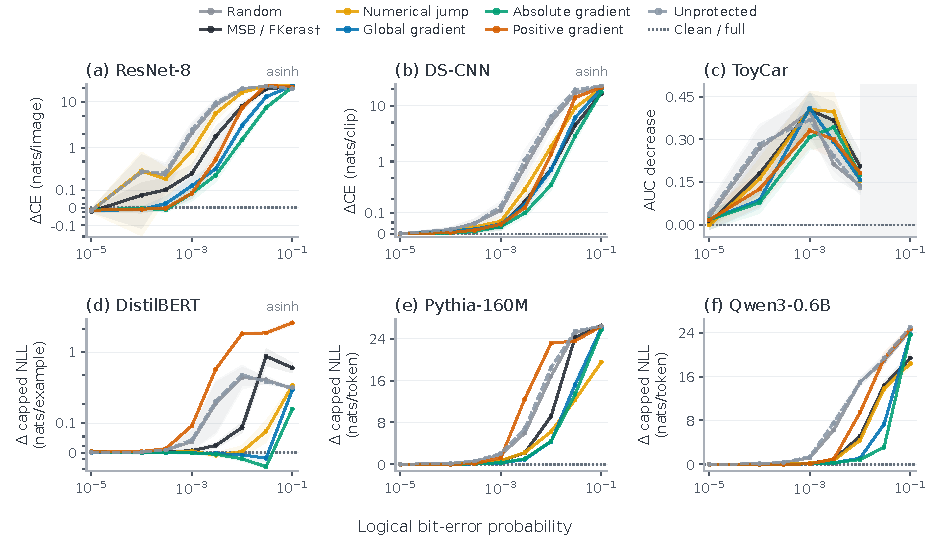
\includegraphics[width=\linewidth]{compact_reliability_ber_125}
\caption{Loss degradation versus BER at 12.5\% protection. Lower is better; bands are 95\% fault-field intervals and zero is clean/full protection. Panels use their own task units. Asinh denotes nonlinear vertical spacing with original-unit ticks. FKeras equals MSB at this complete tier on the three TFLite models only; it is unavailable for the transformers. Lines connect measured points.}\label{fig:ber}
\Description{Six compact panels comparing measured methods over BER, with unprotected and clean references.}
\end{figure}

\begin{figure}[tbp]
\centering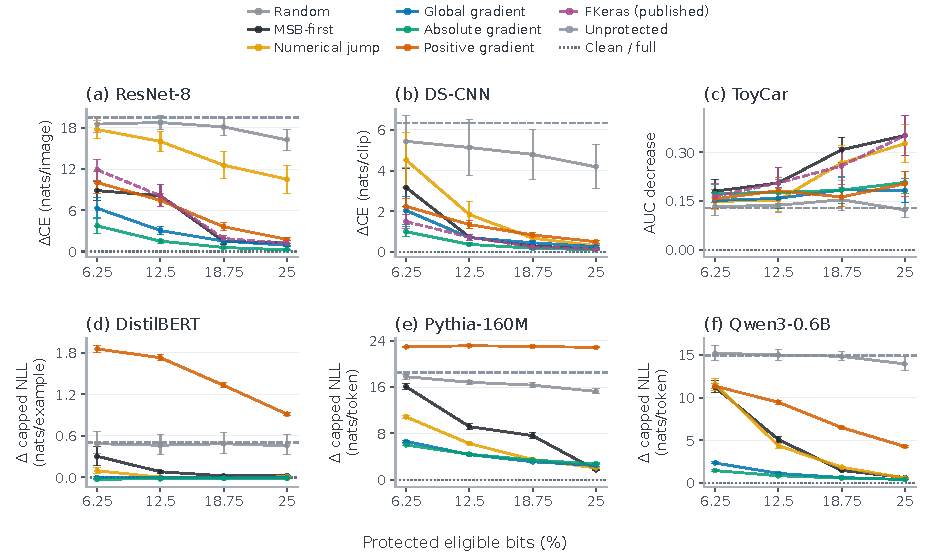
\includegraphics[width=\linewidth]{compact_reliability_budget_001}
\caption{Loss degradation versus protected fraction at BER 1\%. Error bars are 95\% field-level mean intervals. Horizontal references show unprotected and clean/full protection. Equal fractions refer to different eligible-bit populations, not equal hardware cost or absolute fault exposure.}\label{fig:budget}
\Description{Six compact budget panels including the partial-tier comparisons and task-specific uncertainty.}
\end{figure}

\subsection{Changes in method preference}
Paired contrasts, rather than overlapping marginal bands, establish the reversals in Table~\ref{tab:paired}. On Pythia, global gradient is better than MSB-first at 12.5\% coverage but worse at 25\%, for the same checkpoint, BER and cohort. At partial tiers, the Hessian-based allocation is better than MSB-first on KWS and worse on ResNet-8. At complete tiers their masks and outcomes coincide, so they are not independent alternatives.

\begin{table}[t]
\caption{Paired loss differences at explanatory conditions. Negative favors the first method. Units are nats per image, clip, or token. Original Holm families are retained; Qwen follow-up intervals are exploratory. Full grids accompany the paper.}\label{tab:paired}
\centering\small
\begin{tabularx}{\linewidth}{l r r X r}\toprule
Model; contrast & BER & Budget & Difference [95\% CI] & Holm $p$\\\midrule
KWS; FKeras $-$ MSB & .01 & 6.25\% & $-1.678$ [$-2.425,-.930$] & .0112\\
ResNet-8; FKeras $-$ MSB & .01 & 6.25\% & $+3.035$ [$1.835,4.234$] & .0112\\
Pythia; global $-$ MSB & .01 & 12.5\% & $-4.823$ [$-5.395,-4.343$] & .0160\\
Pythia; global $-$ MSB & .01 & 25\% & $+.771$ [$.553,1.025$] & .0160\\
Qwen; absolute $-$ MSB & .05 & 12.5\% & $-9.297$ [$-10.021,-8.567$] & ---\\
Qwen; absolute $-$ MSB & .075 & 12.5\% & $+1.637$ [$.605,2.661$] & ---\\\bottomrule
\end{tabularx}
\Description{Opposite paired method preferences across architectures, protection budgets and BERs.}
\end{table}

Qwen's follow-up reversal also appears in finite uncapped NLL: at BER 7.5\%, absolute gradient gives 23.149 versus 21.374 for MSB-first. However, 10.49\% and 7.07\% of finite token losses reach the 30-nat ceiling. The effect is not solely a capping artifact, but occurs under severe degradation. It does not identify a practical operating range or prove an interaction-driven transition.

\subsection{Monte Carlo-guided allocation}
Conditional selection changes the exact-isolated mask in 27 of 32 KWS pools. Its held-out mean difference is nevertheless only $-8.24\times10^{-5}$ nats/clip, with across-pool interval $[-0.00169,0.00153]$ and two-sided $p$-value 0.918 (Fig.~\ref{fig:decisions}). Eleven pools favor conditional selection, five tie and sixteen favor isolation. Thus, the changed decisions do not establish improved expected protection.

\begin{figure}[tbp]
\centering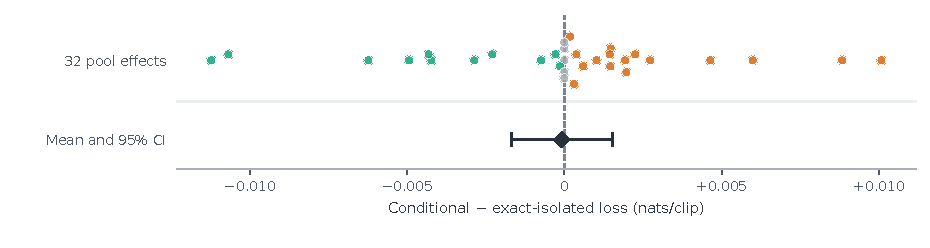
\includegraphics[width=.90\linewidth]{compact_kws_pools}
\caption{Held-out conditional-minus-exact-isolated loss across all 32 KWS pools at BER 5\%. Each dot is one pool; the diamond and bar show the mean and its 95\% pool-level interval. Negative favors conditional selection. Vertical offsets only separate overlapping dots. The mean does not resolve an advantage.}\label{fig:decisions}
\Description{All pool effects around zero, with an unresolved mean improvement and visible heterogeneity.}
\end{figure}

Both methods improve slightly over the original absolute-gradient mask: conditional selection by 0.00268 nats/clip, interval $[0.00058,0.00478]$, and isolation by 0.00248, interval $[0.00036,0.00459]$; both saved Holm-adjusted $p$ values are 0.0279. These separate paired estimates need not subtract exactly. The result supports a benefit from local reevaluation, not a unique benefit from conditioning. Exact interaction diagnostics in the appendix likewise show changed preferences without resolved conditional-over-isolated superiority.

\subsection{Computational cost}
Mean construction times for global gradient are 1.19/0.41/3.85 seconds on ResNet-8/KWS/ToyCar; rank-two Hessian scoring takes 5.58/1.43/11.42 seconds. Shared absolute/positive-gradient computation takes 16.99/7.47/208.43 seconds, excluding loading. Median wide-sweep evaluation times are 23.75, 11.56 and 32.55 seconds per DistilBERT, Pythia and Qwen request. Conditional selection requires $2^K$ evaluations per outside field. Its cost is therefore material even when the measured decision gain is small.

\section{Discussion and Limits}\label{sec:discussion}
\subsection{What a protection designer can conclude}
The results support evaluating a ranking at the intended checkpoint, metric, BER and budget before accepting its allocation. A structural ranking is inexpensive and sometimes competitive; a gradient ranking can produce a large gain in another region. Additional computational sophistication does not impose an ordering on protection quality. FKeras can be better or worse at partial tiers, and at complete tiers its strict ordering produces exactly the same mask as MSB-first. Conditional evaluation can change local decisions without yielding a resolved held-out improvement. NetSuRF makes these alternatives measurable within one explicit contract.

A practical use of the flow is therefore to establish the clean and unprotected references, construct a small set of affordable masks on calibration data, and compare them using paired final fields over the intended operating region. The reported uncertainty determines whether the data support choosing between masks. If a difference is unresolved and the construction costs differ substantially, the experiment supplies no evidence-based reason to prefer the expensive analysis on protection quality alone. This is a decision rule for interpreting evidence, not a proof that one score should always be selected.

\subsection{Reversal is an outcome; interaction is a mechanism}
The Pythia budget reversal and Qwen BER crossover are direct comparisons of frozen masks under paired faults. They establish that an allocation's relative quality can change within one model. They do not separately identify numerical-encoding effects, surrogate approximation error, calibration sensitivity, nonlinear task aggregation, finite-loss clipping, or multiple-fault interactions. Nor does a large variance prove interaction: variable inputs or rare harmful single events can also produce a broad outcome distribution.

The exact response-table diagnostic addresses a narrower mechanistic question. It holds the checkpoint, candidate identities, protection context and selection cohort fixed, and separates clean isolated responses from responses conditioned on outside faults. In those recorded subproblems, the outside context accounts for most of the changed ordering. This supports contextual analysis, while the independent KWS follow-up shows why changed ordering is insufficient evidence of a useful optimizer. The expected benefit can be small compared with selection noise, or the chosen mask can transfer poorly to final fields and inputs.

\subsection{Scope of the fault and resource abstractions}
The study concerns persistent faults in eligible stored parameters. It does not compare their exposure with activations, accumulators, instructions, quantization metadata or control state. Transient activation injection would require its own location, lifetime, execution and sampling contract. Adding such a study could broaden coverage, but a weight-storage experiment cannot establish its results by analogy. Likewise, logical BER does not specify a radiation environment. The high-BER arms are stress tests, and a device-level deployment would require a mapping from physical faults and repair behavior to this software model.

Equal protected fractions are equal fractions of the \emph{declared population}, not equal storage overheads or equal expected task benefit. The INT8 populations span more than four orders of magnitude. Even at the same $p$ and $c$, the expected applied count $(N-B)p$ and the role of each coordinate differ. The restricted FP32/BF16 pilots remain separate evidence and are not combined with these full-eligible INT8 grids. No quantitative claim about physical ECC, TMR, ABFT or Ranger follows from the ideal masks.

\subsection{External validity and missing comparisons}
Each main result is conditional on one frozen checkpoint and a bounded input cohort. Fields quantify fault randomness; they do not replicate training or data collection. The language-model evaluation windows are particularly small relative to the full corpus, and severe corruption encounters an explicit loss cap. The Qwen crossover retains a reversal in the finite uncapped diagnostic, but this does not remove its post-hoc design history or saturation risk. The Pythia high-BER cap-frequency omission limits mechanistic interpretation of its highest-loss conditions.

Method coverage is also incomplete. Published-form FKeras is measured on all three smaller models, with a bounded eigenpair approximation and model-specific continuous loss. Its unavailable transformer results cannot be inferred from inference support. PrioriFI-derived allocation requires a validated ranking-to-protection contract and independent effectiveness evidence; the present engineering implementation does not supply that comparison. These gaps constrain any claim that the measured methods span the best available allocations.

The principal new contribution is the controlled software evaluation and the protection-decision evidence it enables. Selective hardening, gradient sensitivity, feedback-guided injection and context-dependent layer diagnostics already exist~\cite{guo2025inpixel,weng2024fkeras,weng2026priorifi,alobaidi2026selectiveecc}. The present results extend the comparison across exact storage populations, numerical backends and task metrics, and test a conditional alternative against exact isolated selection rather than only a weak structural baseline. They do not establish a universal dynamic optimizer or a first discovery of neural-network interactions.

\section{Conclusion}\label{sec:conclusion}
We presented NetSuRF as a software design flow for assessing budgeted bit protection in quantized neural networks. The flow connects exact encoded-state perturbations, explicit susceptibility definitions, immutable masks, common random fault fields and task-specific evaluation. Its output is a measured reliability landscape indexed by checkpoint, ranking, protection budget and logical BER.

The six-model evaluation shows that protection quality can change substantially with the operating condition. Paired Pythia results reverse the global-gradient versus MSB comparison as the budget changes, and a separate Qwen diagnostic reverses the absolute-gradient comparison as BER increases. Published-form FKeras adds useful partial-tier comparisons on the three smaller models, while complete-tier masks expose exact equivalences that should not be mistaken for independent methods. ToyCar demonstrates the need to preserve the application metric when a differentiable ranking uses a different surrogate objective.

Exact conditional analysis explains why isolated damage has no general allocation guarantee, but the bounded KWS follow-up also establishes the limit of the present alternative: changing many local decisions did not resolve a held-out gain over exact isolated selection. The engineering conclusion is to measure the protection decision under its declared conditions and to report its uncertainty and construction cost. A static mask remains a valid deployment choice; its value is established by the task and fault context in which it is evaluated.

\begin{acks}
AI-assisted tools supported software development, evidence organization, statistical re-analysis, figure preparation and drafting. The scientific claims in this manuscript are linked to the archived measurements and derivations identified in the accompanying evidence manifest. Responsibility for the submitted work rests with the authors.
\end{acks}
\bibliographystyle{ACM-Reference-Format}
\bibliography{references}
\appendix
\section{Probability Identities and Approximation Limits}\label{app:proofs}
\subsection{Protection benefit and equal-budget swaps}
Let $G$ exclude an unprotected bit $b$. Independence gives
\[
J_p(\protset)=(1-p)\E R(G)+p\E R(G\cup\{b\}),\qquad
J_p(\protset\cup\{b\})=\E R(G).
\]
Subtracting proves Eq.~\eqref{eq:protection-benefit}. For the swap in Eq.~\eqref{eq:swap}, the old mask leaves $b$ exposed and the new mask leaves $a$ exposed. Both share the same Bernoulli background and no-fault term; subtracting yields the stated result. These are elementary conditioning identities. They do not require additive loss, differentiability or a neural network. They also do not identify naturally absent faults with interventions under arbitrary correlated or fixed-count laws.

For additive risk $R(A)=R(\varnothing)+\sum_{b\in A}I_b$, linearity gives $J_p(\protset)=R(\varnothing)+p\sum_{b\notin\protset}I_b$. Equal-cost, equal-probability exact-budget optimization therefore selects the largest $I_b$. The nonadditive counterexample in Sec.~\ref{sec:allocation} is nonnegative on all eight states and changes the optimal budget-one mask at $p=1/15$. It proves failure of a general guarantee, not failure for every network.

\subsection{Exact candidate interactions and a useful caution about bounds}
For a fixed outside field, the Boolean response has the unique multilinear expansion~\cite{odonnell2014analysis}
\[
h_G(A)=\sum_{T\subseteq A}\mu_G(T),\qquad
\mu_G(T)=\sum_{U\subseteq T}(-1)^{|T|-|U|}h_G(U).
\]
Thus $J_G(Q)=\sum_{T\subseteq C\setminus Q}p^{|T|}\mu_G(T)$, and the order-one truncation is precisely the outside-conditioned additive part of Eq.~\eqref{eq:decomposition}. Signed coefficients can cancel. A sum of absolute coefficient magnitudes is a bound or diagnostic, not the signed protection benefit. Boolean multilinear expansions and their expectation identities are established mathematics, not new foundations introduced by NetSuRF.

Suppose $h_G(A)\in[a,a+M]$ and $n=|C\setminus Q|$. The order-one prediction for a state with $s\ge2$ candidate faults is $\sum_{b\in A}h_G(\{b\})-(s-1)h_G(\varnothing)$. Its deviation from $h_G(A)$ is at most $sM$, while it is exact at $s=0,1$. For $S\sim\mathrm{Binomial}(n,p)$,
\begin{equation}\label{eq:bound}
\left|J_G(Q)-h_G(\varnothing)-p\sum_{b\in C\setminus Q}d_b^G\right|
\le M\E[S\mathbf1_{S\ge2}]
=Mnp\left[1-(1-p)^{n-1}\right].
\end{equation}
This gives $O(n(n-1)p^2)$ behavior at fixed small $n$ and low $p$. AUC risk has $M=1$; a valid bounded-loss range is needed for other tasks. The bound may be far too loose to certify an allocation because observed decision gaps can be much smaller. It bounds residual \emph{within-candidate} interactions after conditioning on the outside field; it says nothing comparable about the error of clean isolated scores caused by a large faulty background. Uniform risk approximation error $\varepsilon$ would imply at most $2\varepsilon$ excess risk for its minimizer over the same feasible set, but the present empirical studies do not establish a useful whole-network $\varepsilon$.

\section{Additional Evidence and Reproducibility Boundaries}\label{app:evidence}
The companion figure supplement supplies all four measured interior budgets for all six models. Machine-readable condition means, paired contrasts, cohort identities, source manifests, score-construction receipts and figure scripts are distributed separately. Each table or panel is traced to a finalized scientific payload; checksums and development identifiers are kept out of the reader-facing plots.

The earlier conditional attribution study includes a 12-pool KWS study at BER 0.01, a separate 12-pool KWS sweep at 0.001, 0.003 and 0.01, four ResNet-8 pools at 0.01, and four ToyCar pools at 0.001. Pool identities are reused across BER where specified and must not be counted as independent samples of architecture. Table~\ref{tab:attribution} compares strict mask-order reversals against the full response-table selection objective. Counts are dependent pairwise order comparisons, not independent statistical trials. All six saved across-pool held-out selected-minus-isolated intervals include zero.

\begin{table}[h]
\caption{Selection-order reversals relative to the exact response table. Conditioning individual candidate effects on outside faults removes most recorded reversals in these bounded designs. These counts do not establish held-out superiority.}\label{tab:attribution}
\centering\small
\begin{tabular}{llrr}\toprule
Model & BER & Clean additive & Outside-conditioned additive\\\midrule
KWS, initial pools & 0.01 & 396 & 8\\
KWS, multi-BER pools & 0.001 & 328 & 0\\
KWS, multi-BER pools & 0.003 & 305 & 0\\
KWS, multi-BER pools & 0.01 & 376 & 4\\
ResNet-8 & 0.01 & 201 & 1\\
ToyCar & 0.001 & 196 & 0\\\bottomrule
\end{tabular}
\Description{Full selection-order attribution for six historical model and BER groups, preserving negative and unresolved held-out findings.}
\end{table}

Additional bounded scaling studies on KWS and ResNet-8 examined candidate sizes 6, 12, 32 and 64 at three expected-fault levels, with four pools per condition. Exact selection was feasible only at the smaller sizes. At sizes 6 and 12, the outside-conditioned additive choice had zero recorded selection regret against the restricted exact choice in all 24 conditions per model. This is finite-table agreement, not a theorem about larger pools. All 54 simultaneous equal-pool intervals per model included zero; several differences were identically zero, which does not establish population equivalence. These measurements do not support a scalable optimizer-superiority claim. They help identify where expensive exact enumeration currently adds little observed decision value.

\subsection{Historical estimators and precision-specific studies}
Separate focused follow-ups strengthen two partial-tier comparisons without being pooled into the main grid. On ResNet-8 at $p=0.01$ and 6.25\% coverage, 320 paired fields give FKeras minus MSB cross-entropy $+2.241$ nats/image, interval $[1.890,2.593]$, in the same direction as the main study. On ToyCar at $p=0.01$ and 18.75\% coverage, 384 paired fields give FKeras minus absolute-gradient AUC risk $+0.1106$, interval $[0.0920,0.1292]$. Both retain their saved Holm-adjusted $p=0.0012$. These follow-ups improve fault-field precision conditional on their existing cohorts and masks, not generalization to new trained models.

The historical qPolarGrad code is preserved under its recovered definition. The extra factor in the old printed expression is documented rather than silently repaired. Its prior hardware-flow results are not reintroduced as matched evidence for the present checkpoints. Earlier FP32/BF16 studies, including the 96-bit language-model pilots and 1,024-bit DistilBERT classifier subset, remain separate restricted-universe evidence. They are not pooled with full-eligible INT8 curves or counted as independent architecture confirmations. Their representation effects and selection geometry require their own claims and controls.

\subsection{Remaining generalization requirements}
The main curves use one frozen checkpoint per model. Multiple fault fields quantify conditional fault randomness; they do not replace new checkpoints, independently sampled evaluation cohorts or repeated ranking construction. Published FKeras is missing from the transformer grids, and no matched PrioriFI-derived effectiveness grid is included. A stronger allocation claim requires a prespecified comparison against these feasible baselines, separate mask-construction and final-evaluation information, and uncertainty over the intended deployment populations. Those are prospective requirements, not unreported results.

\end{document}
